\documentclass[12pt,a4paper]{report}
\usepackage[english]{babel}
\usepackage[utf8]{inputenc}
\usepackage[T1]{fontenc}
\usepackage{amsmath, amssymb}
\usepackage{graphicx}
\graphicspath{{figures/}}
\usepackage{booktabs}
\usepackage{subcaption}
\usepackage{hyperref}
\usepackage{geometry}
\geometry{margin=1in}
\usepackage{float}
\usepackage{placeins}
\usepackage{soul}
\usepackage{xcolor}
\sethlcolor{yellow}

\begin{document}
\frenchspacing
\hypersetup{pageanchor=false}
\pagenumbering{roman}

% Title Page
\begin{titlepage}
    % UDS logo on the top-left
    \noindent
    \begin{minipage}[t]{0.5\textwidth}
        \raggedright
        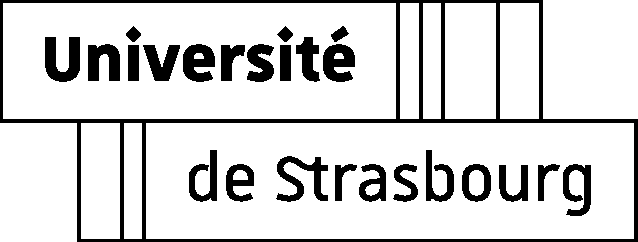
\includegraphics[width=0.7\linewidth]{logo-uds.pdf}
    \end{minipage}
    \hfill
    % iCube logo on the top-right
    \begin{minipage}[t]{0.5\textwidth}
        \raggedleft
        
\includegraphics[width=0.6\linewidth]{icube.pdf}
    \end{minipage}

    \vspace{3cm} 

    \begin{center}
        {\Huge \bfseries Feature superposition and interference in convolutional neural networks\\\par}
        \vspace{2cm}
        
        {\Large \textbf{TER Master 1}\\
        Sciences de données et systèmes complexes\par}
        {\large Université de Strasbourg\par}

        \vspace{3cm}

        % Author + Supervisor
        {\large \textbf{Author:} \\ Yasmina FARID \par}
        \vspace{1cm} 
        {\large \textbf{Supervisor:} \\Anne JEANNIN-GIRARDON\par}
        \vfill
        {\large May 2026}
        
    \end{center}
\end{titlepage}

\setcounter{page}{2}

% Abstract Page
\thispagestyle{plain}
\vspace*{\fill}
\begin{center}
    \Large\textbf{Abstract}
\end{center}
\vspace{0.8cm}

This work examines how the design of convolutional neural network blocks may be linked
to superposition and interference in learned representations. It builds on prior research
on the superposition phenomenon in neural networks as well as on studies of lightweight
and bottleneck-based convolutional architectures, in order to understand how architecture
can influence the internal organization of features inside a CNN. In this context, it
contributes an empirical comparison of three small models: a baseline CNN, a standard
bottleneck model, and an inverted bottleneck model. Their internal representations are
analyzed using cosine similarity and effective rank, in an attempt to approximate
superposition through indirect measures, since this remains an unresolved challenge. The
results show that the three architectures do not organize information in the same way:
the standard bottleneck shows stronger representational concentration and the strongest
individual channel alignment, while the inverted bottleneck keeps the representations
more spread out. The baseline shows that channel overlap can also occur without an
explicit bottleneck. Overall, the work suggests that architectural choices may be related
to differences in how features are represented inside a CNN, and to different superposition-like
and interference-related conditions.

\vspace*{\fill}
\clearpage

% Table of Contents
\tableofcontents
\clearpage

\hypersetup{pageanchor=true}
\pagenumbering{arabic}

% Introduction
\section{Introduction}

\subsection{Context}
Convolutional Neural Networks (CNNs) have become central to modern computer vision. Their effectiveness comes largely from the convolution operation, which captures local spatial patterns efficiently through weight sharing. However, convolution is not a single fixed mechanism. CNNs are composed of sequences of convolutional blocks with varying designs, which means that they do not process features in the same way. These architectural differences influence how features are extracted, combined, and compressed, affecting not only computational efficiency but also how information is internally structured during training.

Understanding these internal representations has become a key focus in interpretability research. One important phenomenon in this area is \textit{superposition}, where a network encodes more features than its dimensionality would normally allow by overlapping them within shared directions of the activation space. While efficient, this strategy can introduce interference when features co-occur, degrading representation quality and making interpretation more difficult.

\subsection{Motivation}
Recent work has focused on developing lightweight CNN architectures that maintain strong performance while reducing parameter count, computational cost, and memory usage, especially for deployment on resource-constrained devices such as mobile or embedded systems (Liu et al.~\cite{liu2024}). These efficiency gains are closely tied to architectural design choices, particularly in convolutional blocks, making them an important point of study for representation analysis.

At the same time, CNN architectures present a significant structural diversity. Younesi et al.~\cite{younesi2024} emphasize that analyzing these architectural differences is essential for understanding their respective strengths, limitations, and application domains. This suggests that architectural design is not only a technical choice but also a factor shaping how information is organized within the network.

This question becomes especially relevant in low-parameter models, where architectural constraints are stronger and design choices have a more pronounced effect. Hollard et al.~\cite{hollard2025} show that bottleneck-based architectures differ not only in accuracy and scaling behavior but also in their reliance on interference across designs. This connects to superposition, as interference can be viewed as a consequence of overlapping feature representations.

However, it remains unclear how different convolutional block designs influence the internal organization of learned features. This leads to the following research question: \textit{How does convolutional block design influence the geometric organization of internal feature representations in CNNs, and what does this suggest about superposition and interference?}

To address this question, this work implements and analyzes a controlled experiment comparing three architectures: a channel-matched baseline CNN, a standard bottleneck CNN, and an inverted bottleneck CNN. All models are trained on a four-class subset of CIFAR-10. Their internal representations at the second block are analyzed using cosine similarity and effective rank to evaluate differences in feature organization.

\clearpage

% Chapter 1: State of the Art
\chapter{State of the Art}

\section{Superposition and interference}

\subsection{Polysemanticity as a structural constraint}

Polysemanticity is a phenomenon in which a neural network encodes multiple distinct
features within a single neuron, in order to store more features than its available dimensions would normally allow. The idea that networks may do this is not novel in itself, it
has been pointed at in many research papers working on interpretability. Elhage et al.\cite{elhage2022}
explored the superposition phenomenon in depth through experiments on several simple
ReLU-based architectures, which they referred to as toy models.
In practice, polysemantic neurons are observed to form during training when the
model detects more useful features in the input than it has latent dimensions to represent separately. Ideally, features would be represented as orthogonal to one another
in the latent space so that each neuron activation corresponds to a unique direction or
dimension, it is what we call monosemantic neurons. The reason networks instead develop polysemantic neurons is to adapt to the dimensional constraint by packing multiple
feature representations into the same neurons. The superposition is how this is achieved.
It occurs when a neural network stores multiple features within the same activation space
rather than giving each feature its own unique direction. This is possible because features
can still be distinguished through differences in angle and magnitude.

\subsection{Role of sparse features in enabling superposition}

A central finding in Elhage et al. is the key role of feature sparsity in enabling superposition. Sparse features are those that occur rarely and especially rarely at the same
time as each other in a given input. In the toy models, the network learns to place the
representations of such sparse features in the same directions as more frequent or important features for a neuron and because these sparse features almost never co-occur
at the same time, they can share dimensions without interfering with each other.
This sparsity is precisely what allows the superposition to work : most of the time
each neuron behaves as if it represented only one feature since the sparse one rarely
occurs or co-occurs with the dominant feature. However, superposition comes with a cost:
in the case of rare inputs where sparse features do co-occur, their vector contributions
add up, pushing the activations in unexpected directions thus causing interference that
can degrade the reconstruction quality.

\subsection{Role of nonlinear filtering (ReLU) with superposition}

Nonlinear activation functions such as ReLU – which sets negative pre-activations to zero and keeps positive ones intact – act as a natural filter for interference. When sparse features co-occur, their vector sum pushes pre-activation off the intended direction, ReLU helps correcting that by putting to zero the noisy negatives before passing to the next layer, which helps the network ignore rare interference cases and avoid propagating noise within its layers.\\ 

The combination of sparse features, superposed representations, and nonlinear filtering allows compression beyond linear models like PCA. PCA finds orthogonal directions maximizing variance but ignores features beyond available dimensions. For dense features frequently active together, orthogonal representations work well, and linear models perform fine. But for sparse features sharing directions becomes optimal and allows the network to represent far more features than it has dimensions. 

Elhage et al. compared two toy models: a linear model that projects the input into a hidden space and reconstructs it linearly (down-projection \(h = W x\), then reconstruction \(x' = W^{T} h\)) and a ReLU output model that keeps the same projection step but applies a nonlinear reconstruction (down-projection \(h = W x\), then \(x' = \mathrm{ReLU}(W^{T} h + b)\)).\\

The results showed that the linear model always learned only the top-\(m\) most important features as if it was learning the top principal components while the ReLU model trained on sparse features, used superposition to represent more features than it had hidden dimensions, achieving lower reconstruction error while having additional features.\\

Moreover, they showed that models maintain superposition while computing. In their absolute value example computation \(|x| = \mathrm{ReLU}(x) + \mathrm{ReLU}(-x)\), superposition still occurred as gradient descent found solutions that could approximate this computation even when neurons encoded multiple features. This demonstrates that superposition can support computational circuits along with compression.


\subsection{Phase change in superposition enabling}

It has been discovered that superposition doesn’t emerge gradually but through a phase change governed by two parameters: sparsity and the relative feature importance -- the benefit to prediction loss of representing a feature. As sparsity increases and/or relative feature importance grows, the model reaches a threshold where it shifts from representing features orthogonally in dedicated dimensions to storing them in shared ones.

\begin{figure}[H]
    \centering
    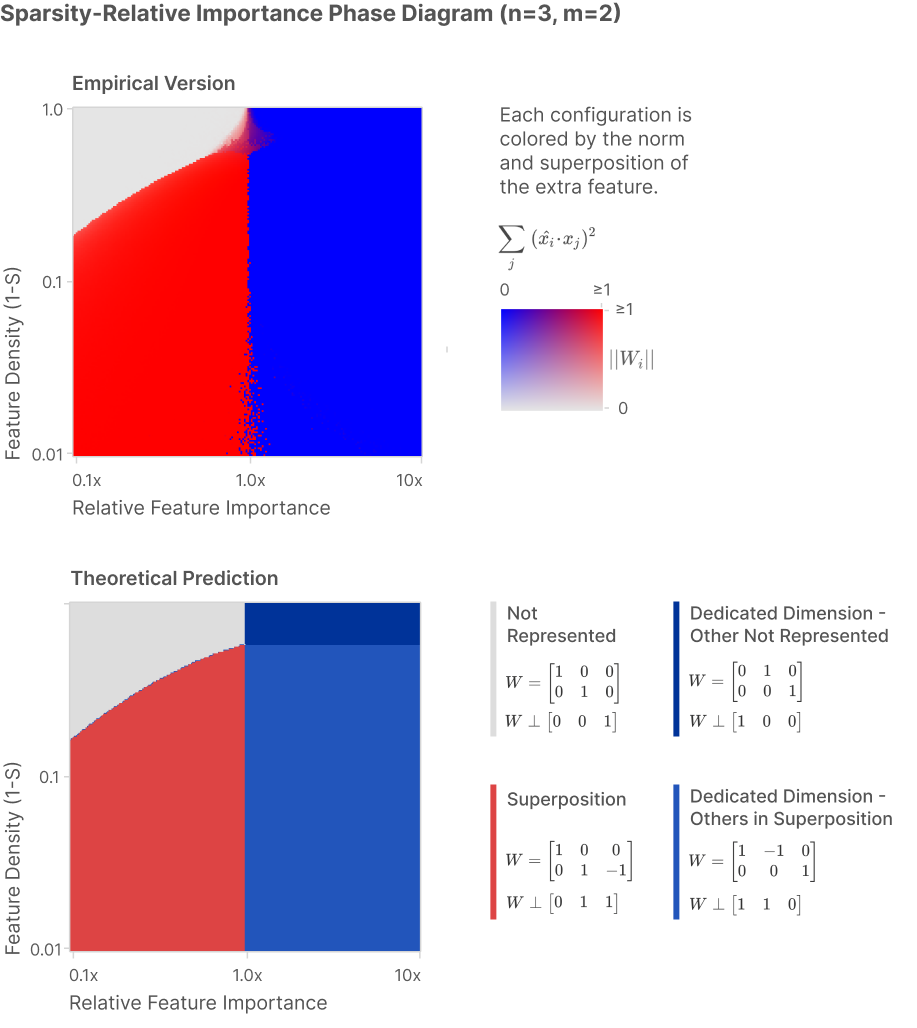
\includegraphics[width=0.7\textwidth]{figures/phase_change.png}
    \caption{Elhage et al. (2022).}
    \label{fig:superposition-phase-change}
\end{figure}

As the phase diagram shows, three outcomes are possible for a given feature: it may not be learned at all; it may be learned and stored in superposition; or it may be given a dedicated orthogonal dimension. Sparse features with sufficient relative importance tend to be stored in superposition (red zone), while features with high enough relative importance receive their own dedicated dimension (blue zone), and sparse features with too little importance may simply not be represented at all (grey zone). The boundary between these regions marks an abrupt transition that represents a discontinuous phase change in the model's encoding strategy.
 

\subsection{Interpretability Challenges with superposition }

An important implication of the superposition mechanism is that mechanistic interpretation becomes very challenging. Ideally for interpretability convenience, if each feature of the input had its corresponding neuron, we could track it through the activations of that neuron allowing us to track the precise causal path from input features to final predictions. But with superposition, neurons activations can have different sources as the neuron activates several features, so it would be nearly impossible to track which feature exactly pushed towards a certain prediction or not. 


\section{Feature representation and architectural design}
The previous sections show that feature representations are shaped by dimensional constraints, sparsity, and nonlinear filtering.his raises the question of whether different convolutional architectures impose these constraints in different ways, and therfor make some of them more likely than others to create, reduce, or reshape such constraints.

In convolutional neural networks, block design determines how features are extracted, combined, and propagated across layers,band since superposition and interference may depend not only on the number of available dimensions but also on whether a block tends to keep features separate or mix them across channels, it is useful to first understand the convolution operations used inside blocks before moving on to the architectures built from them.

\subsection{Convolutional operations}

\subsubsection{Standard convolution}
In the baseline case, a standard convolution is an operation in which a \(K \times K\) kernel slides over the input feature maps, computing weighted sums over local spatial regions and mixing information across channels in a single step~\cite{younesi2024}. This produces output feature maps that capture local patterns such as edges, textures, and shapes. In the survey context, standard convolution is the traditional convolutional layer from which more efficient alternatives have emerged.

\subsubsection{Depthwise convolution}
In contrast, a depthwise convolution applies a separate spatial filter, for example \(3 \times 3\), to each channel independently. Each feature map is processed on its own, producing filtered outputs such as \(FM_1^{\text{conv}}, FM_2^{\text{conv}}, \dots\), while preserving the number of channels. This operation focuses on extracting spatial patterns within each channel, without mixing information between them.

\subsubsection{Pointwise convolution}
A pointwise convolution is a \(1 \times 1\) convolution that operates across channels at each spatial location. At a given position \((i,j)\), it takes the values from all feature maps at that location, \(FM_1(i,j), FM_2(i,j), \dots, FM_n(i,j)\), and computes a weighted sum:
\[
\text{Output FM}(i,j)= w_1\,FM_1(i,j) + w_2\,FM_2(i,j) + \dots + w_n\,FM_n(i,j).
\]
This produces a single output value at that position.This operation is repeated across all spatial locations. Using one pointwise kernel produces one output feature map, while \(K\) kernels produce \(K\) output maps. Its main role is to mix channel information, enabling the network to create new feature combinations or adjust the number of channels. In the context of superposition, this matters because interference arises when different features share the same representational directions, and mixing channels at the same spatial position can make such overlap more likely.

\subsubsection{Depthwise separable convolution}
Depthwise separable convolution factorizes standard convolution into two steps. First, a depthwise convolution extracts spatial features independently for each channel. Then, a pointwise convolution mixes the resulting feature maps across channels. This decomposition separates spatial processing from channel mixing, which significantly reduces the number of parameters and computational cost compared to standard convolution while maintaining strong representational power. As a result, depthwise separable convolutions are widely used in resource-constrained environments such as mobile or embedded vision systems~\cite{younesi2024}.

\subsection{Convolutional block architectures}
Convolutional block architectures provide a higher-level view of how convolution operations are organized within a network. While individual operations determine how information is extracted and mixed locally, block design determines how these operations are combined across layers.

This makes block architectures relevant for studying superposition and interference, since they influence how features are compressed, separated, or recombined. In this work, the scope is restricted to bottleneck-based blocks, which provide a concrete setting for studying representational overlap.

\section{Superposition in bottleneck-based models}

\subsection{Bottleneck architectures}

\subsubsection{Standard bottleneck}
A bottleneck architecture uses a sequence of convolutional operations to transform the channel space. A standard bottleneck first reduces the number of channels with a \(1 \times 1\) convolution, then applies a regular convolution, for example \(3 \times 3\), and finally expands the channels again with another \(1 \times 1\) convolution.

\subsubsection{Inverted bottleneck}
In contrast, the inverted bottleneck first expands the channels using a \(1 \times 1\) convolution. It then applies a depthwise \(3 \times 3\) convolution in the expanded space before reducing the channels at the end. This design is used in MobileNetV2-like models and allows spatial processing in a wider intermediate space while keeping the final representation compact~\cite{hollard2025}.

\subsection{Interference dependence in different bottleneck architectures}
Elhage et al.'s work suggests that dimensional compression and nonlinear filtering can create conditions favorable to superposition. Bottleneck architectures are therefore a relevant case study, because they deliberately compress or expand the channel space inside a block. A recent study approached superposition from an indirect angle: instead of measuring it directly, it constrained the interference that accompanies it by using a superlinear activation called SoLU. SoLU multiplies each activation by its softmax weight across the layer, so that larger activations are emphasized while smaller competing activations are suppressed:
$$\mathrm{SoLU}(x_i)=x_i \cdot \mathrm{softmax}(x)_i = x_i \cdot \frac{e^{x_i}}{\sum_j e^{x_j}}$$
This makes it possible to distinguish architectures that rely on interference from those that remain relatively stable when interference is reduced~\cite{hollard2025}.

The main observation was that not all bottleneck-based architectures respond in the same way to this interference constraint. Models such as MobileNetV2 (inverted bottleneck), MobileNetV3---an improved version of MobileNetV2---and MobileNeXt, all relying primarily on inverted bottleneck designs, lose a significant amount of accuracy when SoLU is applied together with batch normalization~\cite{hollard2025}. This suggests that, in low-parameter settings, their performance benefits from interference rather than relying on fully independent channels, which is consistent with previous findings showing that superposition can outperform linear models in similar situations\cite{elhage2022}.

This finding motivates studying bottleneck design as an architectural variable. If different bottleneck designs change how much a model relies on interference, they may also affect the geometry of the learned feature maps.

\clearpage

% Chapter 2: Experimental Comparison
\chapter{Experimental comparison of bottleneck architectures}

\section{Context}
Building on the theoretical discussion in the previous chapter, this chapter examines whether bottleneck design leads to measurable differences in internal feature geometry. Elhage et al.~\cite{elhage2022} show that superposition can arise when sparse features are represented in shared, non-orthogonal directions, creating interference when overlapping features co-activate. Hollard et al.~\cite{hollard2025} provide the architectural motivation for this study by suggesting that low-parameter bottleneck-based vision models do not all rely on interference in the same way. This motivates comparing bottleneck designs directly rather than assuming that all compact CNNs behave similarly. The goal here is not to prove superposition directly, but to test whether different bottleneck designs produce different patterns of organization in their feature maps. The experimental question is therefore: \textit{Do standard and inverted bottleneck blocks produce different levels of channel overlap and effective representational dimensionality compared with a channel-matched baseline ? and are these patterns consistent with superposition-like feature organization?}

\subsection{Compared architectures}

\subsubsection{Baseline architecture: channel-matched reference}
The reference model is a baseline CNN composed of two regular convolutional blocks without any explicit bottleneck. Its second block returns 8 channels, as in the two bottleneck variants, so that the architectures can be compared at the same measured channel dimension.

\begin{verbatim}
BaselineConvNet: 3 -> 8 -> 8 channels (two ConvBlock layers)
- Block 1: 5x5 conv (k=5) -> 8 channels + BatchNorm + ReLU + MaxPool
- Block 2: 3x3 conv (k=3) -> 8 channels + BatchNorm + ReLU + MaxPool
- Measured block 2 output: [B, 8, 6, 6]
\end{verbatim}

Inside the second block, the baseline applies a single regular convolution, whereas the other two models introduce an intermediate transformation of the channel space. This provides a direct reference for comparing the effect of introducing a bottleneck structure.

\subsubsection{Standard and inverted bottleneck architectures}
To test the bottleneck effects and be able to compare channel-level representations, both variants are also set to return exactly 8 output channels at the measured block.

\begin{verbatim}
StandardBottleneck: 8 -> 4 -> 8 channels
- 1x1 pointwise convolution (reduce: 8 -> 4)
- 3x3 standard convolution (4 channels)
- 1x1 pointwise convolution (expand: 4 -> 8)
- Measured block 2 output: [B, 8, 14, 14]
\end{verbatim}

\begin{verbatim}
InvertedBottleneck: 8 -> 16 -> 8 channels
- 1x1 pointwise convolution (expand: 8 -> 16)
- 3x3 depthwise convolution (16 groups)
- 1x1 pointwise convolution (reduce: 16 -> 8)
- Measured block 2 output: [B, 8, 14, 14]
\end{verbatim}

The three models are compared at a layer where they all have the same number of channels: block 2 always outputs \(C = 8\) channels. However, they are not strictly matched in spatial resolution or parameter count. Because of their design, the bottleneck blocks either reduce or expand the channel dimension within block 2, which changes the number of parameters. Even so, all three models remain small and comparable in overall scale. This table summarizes the measured block in each architecture:

\begin{table}[ht]
\centering
\resizebox{\textwidth}{!}{%
\begin{tabular}{lccc}
\toprule
Architecture & Block 2 Design & Block 2 Output shape & Block 2 Params  \\
\midrule
Baseline      & \(8 \to 8\) standard conv   & \(8 \times 6 \times 6\)   & 600 \\
Standard BT   & \(8 \to 4 \to 8\) reduce-expand        & \(8 \times 14 \times 14\) & 240  \\
Inverted BT   & \(8 \to 16 \to 8\) expand-reduce  & \(8 \times 14 \times 14\) & 480 \\
\bottomrule
\end{tabular}
}
\caption{Architecture summary for the measured second block.}
\label{tab:architectures}
\end{table}

\subsection{Representation measures}
To study how architectural design affects internal feature organization, the experiment uses two complementary measures: effective rank and cosine similarity. Effective rank gives a global estimate of how many directions are effectively used by the learned representation, while cosine similarity measures pairwise directional alignment between channels. Read together, these metrics provide evidence about representational overlap. They do not, however, identify individual semantic features, and therefore cannot diagnose superposition on their own.

\subsubsection{Effective rank of feature maps}
The first measure is the effective rank of the channel activation matrix. This quantity estimates how many independent directions are effectively used by the representation~\cite{roy2007effective}.

Let $X \in \mathbb{R}^{N \times C}$ be the activation matrix obtained by flattening the feature maps of a given layer, where $N$ is the number of collected activation samples and $C$ is the number of channels. Let $\sigma_1, \sigma_2, \dots, \sigma_C$ be the singular values of $X$. We define the normalized singular values as
\begin{equation}
p_i = \frac{\sigma_i}{\sum_{j=1}^{C} \sigma_j}.
\end{equation}

The effective rank is then defined as
\begin{equation}
\mathrm{erank}(X) = \exp\left(-\sum_{i=1}^{C} p_i \log p_i\right).
\end{equation}

This quantity takes values between \(1\) and \(C\). A low effective rank indicates that the representation is concentrated in a small number of dominant directions. A higher effective rank suggests that the channels are distributed across a larger number of effective dimensions. In this study, a lower effective rank may indicate stronger compression or redundancy in the learned feature maps. A higher effective rank may indicate a more distributed representation. The limitation is that effective rank is global: it shows dimensional concentration, but it does not show which features are sharing directions.

\subsubsection{Cosine similarity of feature maps}
Cosine similarity is used as a local measure of directional alignment between channels. It computes the cosine of the angle between two feature vectors rather than relying on their Euclidean distance. By focusing on direction, this metric captures whether two channels produce similar activation patterns, regardless of their magnitude.

Formally, given two channel activation vectors $A$ and $B$ flattened over the collected batch and spatial dimensions, with length $N = B_{\text{total}} \times H \times W$, the cosine similarity $S_C$ is computed as
\begin{equation}
S_C(A,B) = \frac{A \cdot B}{\|A\| \, \|B\|}
= \frac{\sum_{i=1}^{N} A_i B_i}{\sqrt{\sum_{i=1}^{N} A_i^2} \, \sqrt{\sum_{i=1}^{N} B_i^2}}.
\end{equation}

This metric is bounded within the interval $[-1,1]$, providing a clear interpretation of directional alignment:
\begin{itemize}
    \item $S_C = 1$: the vectors point in the same direction, indicating identical feature patterns.
    \item $S_C = 0$: the vectors are orthogonal, implying no similarity between the patterns.
    \item $S_C = -1$: the vectors point in opposite directions, suggesting anti-correlated patterns.
\end{itemize}

\paragraph{Geometric interpretation.}
This geometric interpretation is visualized in Figure~\ref{fig:cosine_sim}, which shows how directionally aligned vectors are grouped within a decision region.

\begin{figure}[ht]
    \centering
    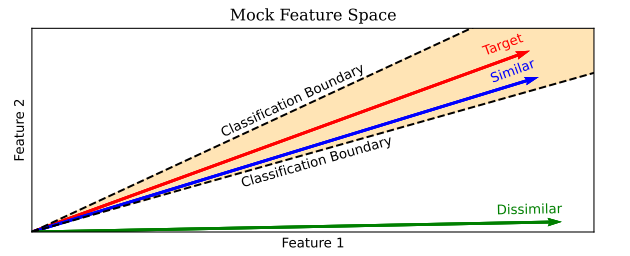
\includegraphics[width=0.9\textwidth]{figures/cosim_def_vis.png}
    \caption{Illustration of cosine similarity in a mock feature space~\cite{falato2022plasma}.}
    \label{fig:cosine_sim}
\end{figure}

As the figure shows, vectors that are directionally aligned, such as Target and Similar, are grouped within a classification boundary, whereas dissimilar vectors are projected far from this region.

In this work, cosine similarity is computed between all pairs of channels in the second block feature maps. For each model, the activations produced by block 2 are collected over the test set, and each channel is flattened across the batch and spatial dimensions. This produces an \(8 \times 8\) similarity matrix whose off-diagonal entries summarize the degree of channel alignment. Large off-diagonal values indicate overlapping activation patterns, which may be compatible with superposition. However, they do not prove superposition, because two channels can be correlated for other reasons, such as shared low-level visual patterns or because the architecture makes some channels learn similar information.

\subsection{Dataset}
The experiment uses a selected subset of CIFAR-10 to ensure that the small models remain appropriate for the task. From the original 60,000 \(32 \times 32\) color images across 10 classes, four classes were selected: automobile (car), bird, cat, and dog. This subset contains 20,000 training images and 4,000 test images:

\begin{verbatim}
- Training set: 20,000 images (5,000 per class)
- Test set: 4,000 images (1,000 per class)
- Classes: car, bird, cat, dog
- Input shape: [64, 3, 32, 32] per batch
\end{verbatim}

\subsection{Training protocol}
All three architectures (channel-matched baseline, standard bottleneck, inverted bottleneck) share the same loss function, optimizer, and batch size:

\begin{verbatim}
Loss function: Cross-entropy loss
Optimizer: Adam (lr = 1e-3)
Batch size: 64
Training duration: 5 epochs
\end{verbatim}

\noindent Data preprocessing used CIFAR-10 standard normalization with mean and standard deviation values from the dataset documentation:
\begin{verbatim}
Mean: (0.4914, 0.4822, 0.4465)
Std: (0.2023, 0.1994, 0.2010)
\end{verbatim}

Training used the standard DataLoader settings with \texttt{shuffle=True}. After training, block-2 feature maps were collected on the test set with the model in evaluation mode. The reported cosine statistics were computed from the off-diagonal entries of the resulting \(8 \times 8\) channel similarity matrix, and the effective rank was computed from the corresponding activation matrix. The models reached similar validation accuracies: 69.5\% for the baseline, 66.8\% for the standard bottleneck, and 69.0\% for the inverted bottleneck. These values are reported only to show that all models learned the task to a comparable degree; accuracy is not the main focus of this experiment.

\section{Results}
Figure~\ref{fig:results_heatmaps} compares the cosine similarity matrices of the Baseline, Standard bottleneck, and Inverted bottleneck models. Since all three models output 8 channels at the measured layer, each matrix has size 8×8. However, the baseline feature maps do not have the same spatial resolution as the bottleneck feature maps. Therefore, the figure should mainly be read as a comparison of how the 8 output channels are organized within each model, rather than as a fully controlled comparison between identical architectures.

\begin{figure}[ht]
    \centering
    {\large\textbf{Cosine Similarity Matrices Across Architectures}}\par
    \vspace{0.3cm}

    % First row: Baseline centered
    \begin{minipage}{0.46\textwidth}
        \centering
        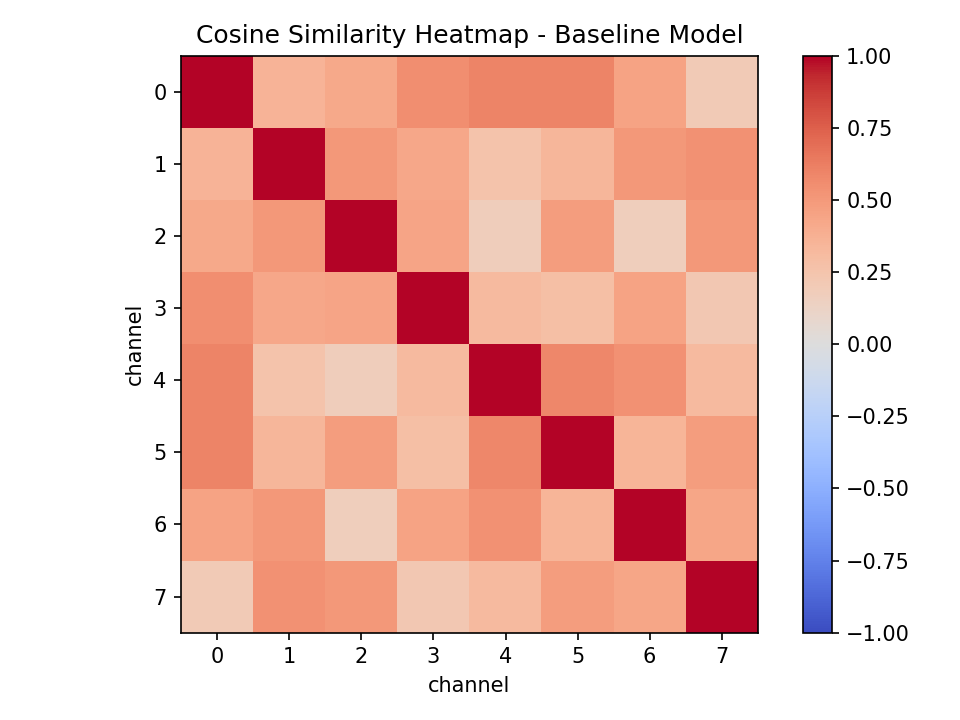
\includegraphics[width=\textwidth]{figures/cosim_bsl.png}
        \subcaption{Baseline}
    \end{minipage}

    \vspace{0.2cm}

    % Second row: Standard BT and Inverted BT
    \begin{minipage}{0.46\textwidth}
        \centering
        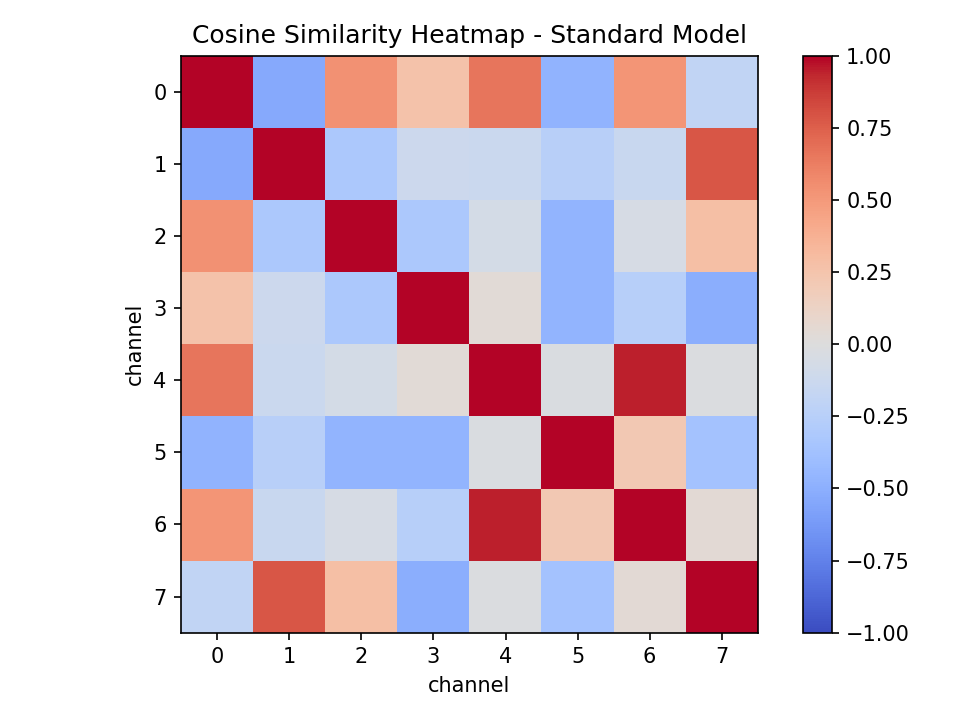
\includegraphics[width=\textwidth]{figures/cosim_std.png}
        \subcaption{Standard Bottleneck}
    \end{minipage}
    \hfill
    \begin{minipage}{0.46\textwidth}
        \centering
        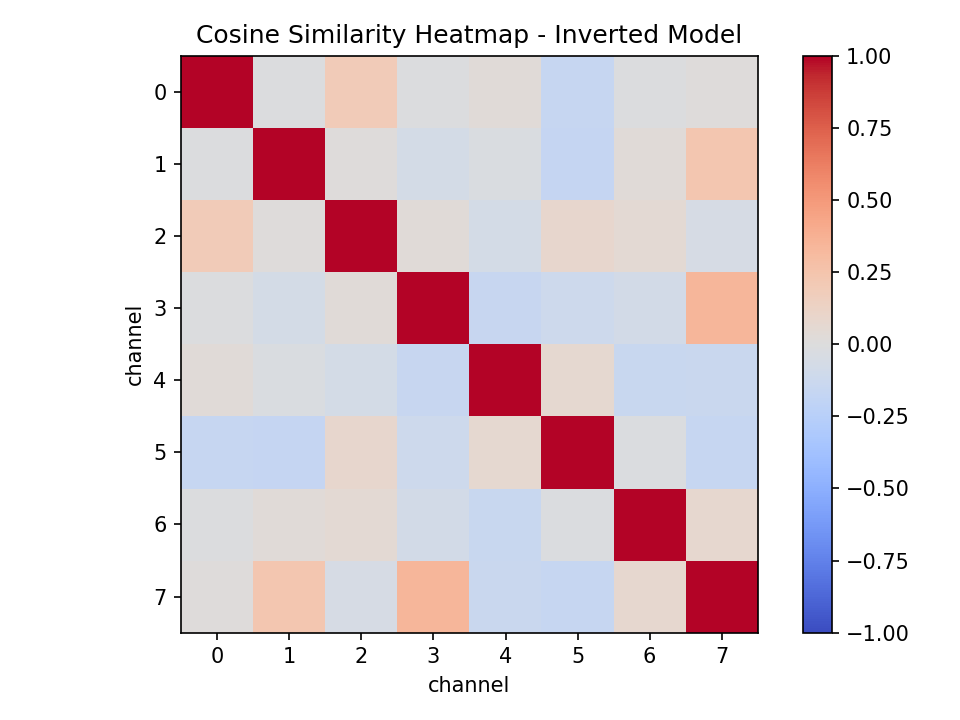
\includegraphics[width=\textwidth]{figures/cosim_inv.png}
        \subcaption{Inverted Bottleneck}
    \end{minipage}

    \caption{Cosine similarity heatmaps for the second block feature maps across architectures.}
    \label{fig:results_heatmaps}
\end{figure}
\FloatBarrier

These visual observations are supported by the quantitative metrics summarized in this table : 

\begin{table}[H]
\centering
\begin{tabular}{lccc}
\toprule
Architecture & Mean Abs Offdiag & Max Abs Offdiag & Frac > 0.5 \\
\midrule
Baseline      & 0.4198 & 0.7063 & 0.2500 \\
Standard BT   & 0.3247 & 0.9199 & 0.2500 \\
Inverted BT   & 0.1450 & 0.4398 & \textbf{0.0000} \\
\bottomrule
\end{tabular}
\caption{Cosine similarity statistics computed from off-diagonal channel pairs.}
\label{tab:results_stats}
\end{table}

To complement this pairwise measure, effective rank was computed from the same block-2 feature maps. Since all measured representations have \(C=8\) channels, the normalized effective rank is obtained by dividing the effective rank by 8. The results are reported in this table : 

\begin{table}[ht]
\centering
\begin{tabular}{lcc}
\toprule
Architecture & Effective Rank & Normalized Effective Rank \\
\midrule
Baseline      & 7.0406 & 0.8801 \\
Standard BT   & \textbf{4.1000} & \textbf{0.5125} \\
Inverted BT   & 7.7319 & 0.9665 \\
\bottomrule
\end{tabular}
\caption{Effective rank statistics computed from block-2 channel activations.}
\label{tab:erank_stats}
\end{table}

\section{Interpretation and Discussion}The cosine similarity results first show that the baseline model already has a relatively high level of channel overlap. In this run, it has the highest mean absolute off-diagonal similarity and the same fraction of channel pairs above 0.5 as the standard bottleneck. This means that channel overlap is not specific to bottleneck architectures in this experiment. Therefore, high cosine similarity cannot be interpreted as direct evidence of superposition, as it can also reflect ordinary correlations between channels, shared low-level visual patterns, or the small size of the model.\\

On the other hand, comparing the two bottleneck architectures still shows clear differences. The standard bottleneck has the strongest alignment, with the highest maximum off-diagonal similarity. This suggests that at least some channel pairs become strongly aligned after the representation is compressed from 8 to 4 channels and expanded back to 8 channels. The inverted bottleneck shows a different pattern: its off-diagonal cosine similarities remain lower, and no channel pair exceeds the 0.5 threshold. This indicates less pairwise channel alignment at the measured layer.\\

The effective-rank results add a more global view. The baseline has a relatively high cosine similarity, but its effective rank remains close to the maximum value of 8. This means that its representation is not globally concentrated into only a few directions, even though some channels are correlated. The standard bottleneck is different: its effective rank is close to 4 effective directions out of 8 channels. This supports the interpretation that its narrow intermediate layer concentrates information into fewer dominant directions. The inverted bottleneck remains close to full effective rank, which is consistent with its lower cosine similarity and suggests a more distributed representation.\\

Together, these two measures give a cautious interpretation of the results. The standard bottleneck shows stronger channel alignment and a lower effective use of dimensions, while the inverted bottleneck keeps lower channel alignment and a higher effective rank. This suggests that the standard bottleneck organizes its representation in a more concentrated way, whereas the inverted bottleneck keeps the representation more distributed. 
Based on the theory discussed in Chapter 1, these geometric differences support the hypothesis that the standard bottleneck tends toward more superposition-like feature organization, while the inverted bottleneck keeps features more distributed.\\

However, this remains only an indirect approximation of superposition, since superposition means that distinct features are encoded in shared non-orthogonal directions. In this experiment, we do not recover individual semantic features, so the results cannot fully confirm that the aligned channels correspond to distinct superposed features. Cosine similarity and effective rank are therefore useful proxy measures: they can suggest whether an architecture tends to concentrate representations into shared directions, which is a regime where superposition may occur according to theory, but they are not complete diagnostic measures of superposition.\\

A few limitations should also be noted. Although the comparison is channel-matched, the spatial resolution is not exactly the same across all models, so the analysis mainly focuses on channel-level organization. In addition, the results come from a single training run and should therefore be interpreted as indicative trends.

\section{Conclusion}
This work studied whether bottleneck design affects channel-level organization in small CNNs. Using cosine similarity and effective rank, the experiment compared a baseline CNN, a standard bottleneck, and an inverted bottleneck.\\

The main result is that the two bottleneck designs do not behave in the same way. The standard bottleneck appears more concentrated, while the inverted bottleneck preserves a more distributed representation. At the same time, the baseline shows that channel overlap can also appear without an explicit bottleneck, so these measures must be interpreted as indirect proxies rather than direct evidence of superposition.\\

Overall, this work suggests that architectural design can shape superposition-like feature organization in CNN representations, but only at the level of geometric tendencies rather than confirmed feature-level superposition. Sparse Autoencoders provide a possible way to go beyond these proxies by moving from channel-level measurements to a more direct feature-level analysis

\section{Perspective: Sparse Autoencoders}

The next step would be to move from geometric proxies to feature-level analysis. While cosine similarity and effective rank describe the shape of the activation space, they do not identify the actual features encoded by the network. Sparse Autoencoders offer a promising direction because they can learn sparse feature dictionaries from neural activations. 
Recent work by Bereska et al.~\cite{bereska2025} proposes using Sparse Autoencoders to measure superposition more directly by estimating how many effective features are represented in a layer. Applying this approach to convolutional feature maps could help determine whether the overlap observed in this report corresponds to genuine feature sharing or only to generic channel correlation. Although this extension was not pursued here, it represents a natural and promising direction for future research
\clearpage

% Bibliography
\bibliographystyle{plain}
\addcontentsline{toc}{chapter}{Bibliography}

\begin{thebibliography}{9}

\bibitem{elhage2022}
Elhage, N., Hume, T., Olsson, C., Schiefer, N., Henighan, T., Kravec, S., Hatfield-Dodds, Z., Lasenby, R., Drain, D., Chen, C., Grosse, R., McCandlish, S., Kaplan, J., Amodei, D., Wattenberg, M., and Olah, C.
\newblock Toy Models of Superposition.
\newblock {\em arXiv}, 2022.
\newblock \url{https://doi.org/10.48550/arXiv.2209.10652}

\bibitem{hollard2025}
Hollard, L., Mohimont, L., Gaveau, N., and Steffenel, L.-A.
\newblock Exploring Superposition and Interference in State-of-the-Art Low-Parameter Vision Models.
\newblock {\em arXiv}, 2025.
\newblock \url{https://doi.org/10.48550/arXiv.2507.15798}

\bibitem{bereska2025}
Bereska, L., Tzifa-Kratira, Z., Samavi, R., and Gavves, E.
\newblock Superposition as Lossy Compression: Measure with Sparse Autoencoders and Connect to Adversarial Vulnerability.
\newblock {\em arXiv}, 2025.
\newblock \url{https://doi.org/10.48550/arXiv.2512.13568}

\bibitem{liu2024}
Liu, Y., Xue, J., Li, D., Zhang, W., Chiew, T. K., and Xu, Z.
\newblock Image recognition based on lightweight convolutional neural network: Recent advances.
\newblock {\em Image and Vision Computing}, 146:105037, 2024.
\newblock \url{https://doi.org/10.1016/j.imavis.2024.105037}

\bibitem{younesi2024}
Younesi, A., Ansari, M., Fazli, M., Ejlali, A., Shafique, M., and Henkel, J.
\newblock A Comprehensive Survey of Convolutions in Deep Learning: Applications, Challenges, and Future Trends.
\newblock {\em IEEE Access}, 12:41180--41218, 2024.
\newblock \url{https://doi.org/10.1109/ACCESS.2024.3376441}

\bibitem{falato2022plasma}
Falato, M. J., et al.
\newblock Plasma image classification using cosine similarity constrained convolutional neural network.
\newblock {\em Journal of Plasma Physics}, 88:895880603, 2022.
\newblock \url{https://doi.org/10.1017/S0022377822000940}

\bibitem{roy2007effective}
Roy, O., and Vetterli, M.
\newblock The effective rank: A measure of effective dimensionality.
\newblock In {\em Proceedings of the 15th European Signal Processing Conference (EUSIPCO)}, pages 606--610, 2007.
\newblock \url{https://infoscience.epfl.ch/record/119465}

\end{thebibliography}

\end{document}
